%% The following is a directive for TeXShop to indicate the main file
%%!TEX root = diss.tex

\chapter{Lexical decision}

%This chapter reports on two experiments done using a lexical decision paradigm to induce auditory perceptual learning in participants.  This paradigm has been most used in the previous literature (Reinisch line of work, McQueen line of work, some kraljic? but I think some other kraljic uses shapes - maybe just for unlearning phase).

\section{Motivation}

This experiment implements a standard lexically-guided perceptual learning experiment with manipulations to lexical bias and attention.

\section{Experiment 1}

In these two experiments, listeners will be exposed to ambiguous productions of words containing a single instance of /s/, where the /s/ has been modified to sound more like /\textesh/ in a lexical decision task. 
In one group, the S-Initial group, the critical words will have an /s/ in the onset of the first syllable, like in \emph{cement}, with no /\textesh/ neighbour, like \emph{shement}.  
In the other group, the S-Final group, the critical words will have an /s/ in the onset of the final syllable, like in \emph{tassel}, with no /\textesh/ neighbour like \emph{tashel}.  
In addition, half of each group will be given instructions that the speaker has a ambiguous /s/ and to listen carefully, following \citet{Pitt2012}.

Given the difference in word response rates depending on position in the word, we would predict that listeners exposed to ambiguous sounds earlier in words would be less likely to accept these productions as words as compared to listeners exposed to ambiguous sounds later in words.  
In addition, given the reliance of perceptual learning on lexical scaffolding, this lower acceptance rate for the former group would lead to a smaller perceptual learning effect as compared to the latter group.

\subsection{Methodology}

\subsubsection{Participants}

One hundred native speakers of English participated in the experiment and were compensated with either \$10 CAD or course credit. 
They were recruited from the UBC student population.  
Twenty additional native English speakers participated in a pretest to determine the most ambiguous sounds.  
Twenty five other native speakers of English participated for course credit in a control experiment.

\subsubsection{Materials}

One hundred and forty English words and 100 nonwords that were phonologically legal in English were used as exposure materials.  
The set of words consisted of 40 critical items, 20 control items and 60 filler words.  
Half of the critical items had an /s/ in the onset of the first syllable and half had an /s/ in the onset of the final syllable.  
All critical tokens formed nonwords if their /s/ was replaced with /\textesh/. Half the control items had an /\textesh/ in the onset of the first syllable and half had an /\textesh/ in the onset of the final syllable.  
Each critical item and control item contained just the one sibilant, with no other /s z \textesh\ \textyogh\ \textteshlig\  \textdyoghlig/.  
Filler words and nonwords did not contain any sibilants.  
Frequencies and number of syllables across item types are in Table~\ref{tbl:expfreq}

\begin{table}
\caption{Mean and standard deviations for frequencies and number of syllables of each item type}
\label{tbl:expfreq}
\centering
\begin{tabular}{ccc}
\toprule
Item type & Frequency & Number of syllables \\
\midrule
Filler words & 1.81 (1.05) & 2.4 (0.55) \\
/s/-initial & 1.69 (0.85)  & 2.4 (0.59)\\
/s/-final & 1.75 (1.11)  & 2.3 (0.47) \\
/\textesh/-initial & 2.01 (1.17) & 2.3 (0.48) \\
/\textesh/-final & 1.60 (1.12) & 2.4 (0.69) \\
\bottomrule
\end{tabular}
\end{table}

Four monosyllabic minimal pairs of voiceless sibilants were selected as test items for categorization (\emph{sack}-\emph{shack}, \emph{sigh}-\emph{shy}, \emph{sin}-\emph{shin}, and \emph{sock}-\emph{shock}).  
Two of the pairs had a higher log frequency per million words (LFPM) from SUBTLEXus \citep{Brysbaert2009} for the /s/ word, and two had higher LFPM for the /\textesh/ word, as shown in Table~\ref{tbl:catfreq}.

\begin{table}
\caption{Frequencies of words used in categorization continua}
\label{tbl:catfreq}
\centering
\begin{tabular}{ccc}
\toprule
Continuum & /s/-word frequency & /\textesh/-word frequency \\
\midrule
sack-shack & 1.11 & 0.75 \\
sigh-shy & 0.53 & 1.26 \\
sin-shin & 1.20 & 0.48 \\
sock-shock & 0.95 & 1.46 \\

\bottomrule
\end{tabular}
\end{table}


All words and nonwords were recorded by a male Vancouver English speaker in quiet room.  
Critical words for the exposure phase were recorded in pairs, once normally and once with the sibilant swapped forming a nonword.  
The speaker was instructed to produce both forms with comparable speech rate, speech style and prosody.

For each critical item, the word and nonword versions were morphed together in an 11-step continuum (0\%-100\% of the nonword /\textesh/ recording, in steps of 10\%) using STRAIGHT \citep{Kawahara2008} in Matlab (The Mathworks, Inc.).  
Prior to morphing, the word and nonword versions were time aligned based on acoustic landmarks, like stop bursts, onset of F2, nasalization or frication, etc.  
All control items and filler words were processed and resynthesized by STRAIGHT to ensure a consistent quality across stimulus items.

\subsubsection{Pretest}

To determine which step of each continua would be used in exposure, a phonetic categorization experiment was conducted.  
Participants were presented with each step of each exposure word-nonword continuum and each categorization minimal pair continuum, resulting in 495 trials (40 exposure words plus five minimals pairs by 11 steps).  
The experiment was implemented in E-prime (cite).  
As half of the critical items had a sibilant in the middle of the word (onset of the final syllable), participants were asked to respond with word or non word rather than asking for the identity of the ambiguous sound, as in previous research \citep{Reinisch2013}.  

\begin{figure}
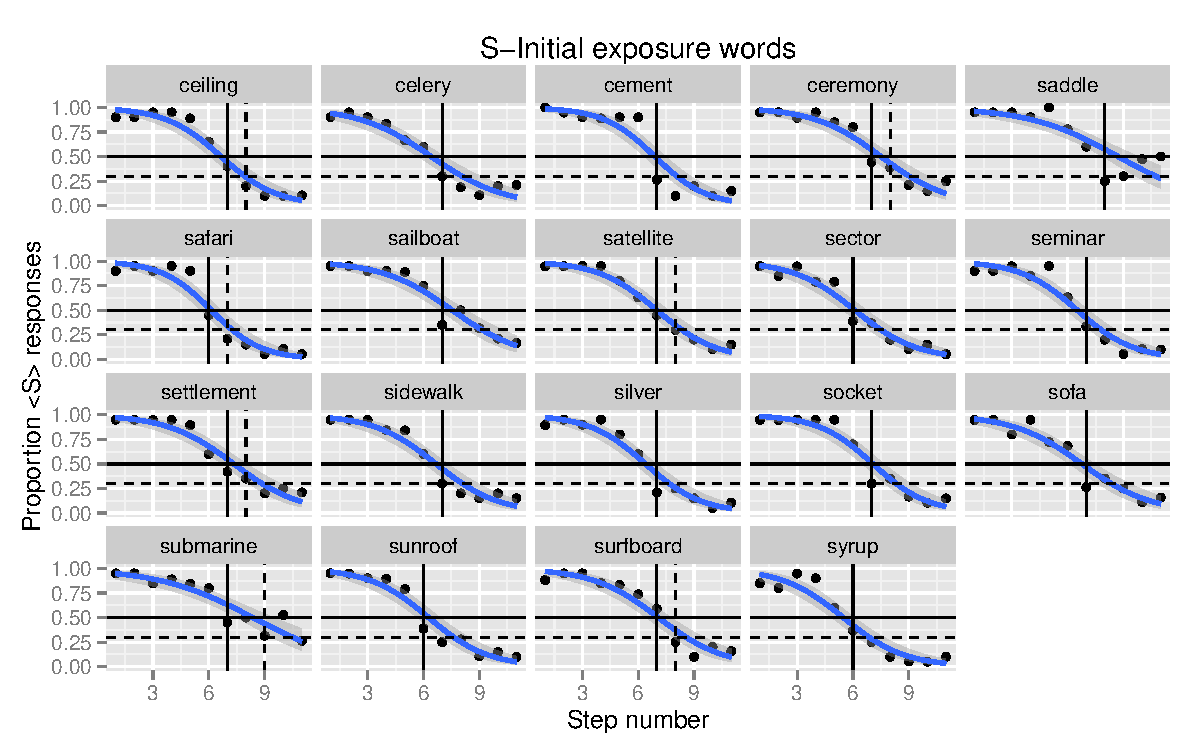
\includegraphics[width=\textwidth]{sinitialpretest.pdf}
\caption{Proportion of word-responses for /s/-initial exposure words. Solid lines represent Experiment 1 selection criteria (50\% word-response rate) and dashed lines represent Experiment 2 selection criteria (30\% word-response rate).  Dots are averaged word-response across subjects, and the blue line is a binomial model constructed from the responses.}
\end{figure}

The proportion of s-responses (or word responses for exposure items) at each step of each continuum was calculated and the most ambiguous step chosen. 
The threshold for the ambiguous step for this experiment was when the percentage of s-response dropped near 50\%. 
A full list of steps chosen for each stimulus item is in the appendix.  For the minimal pairs, six steps surrounding the 50\% cross over point were selected for use in the phonetic categorization task.  
Due to experimenter error, the continuum for \emph{seedling} was not included in the stimuli, so the chosen step was the average chosen step for the /s/-initial words.  
The average step chosen for /s/-initial words was 6.8 ($SD = 0.5$), and for /s/-final words the average step was 7.7 ($SD = 0.8$).

\begin{figure}
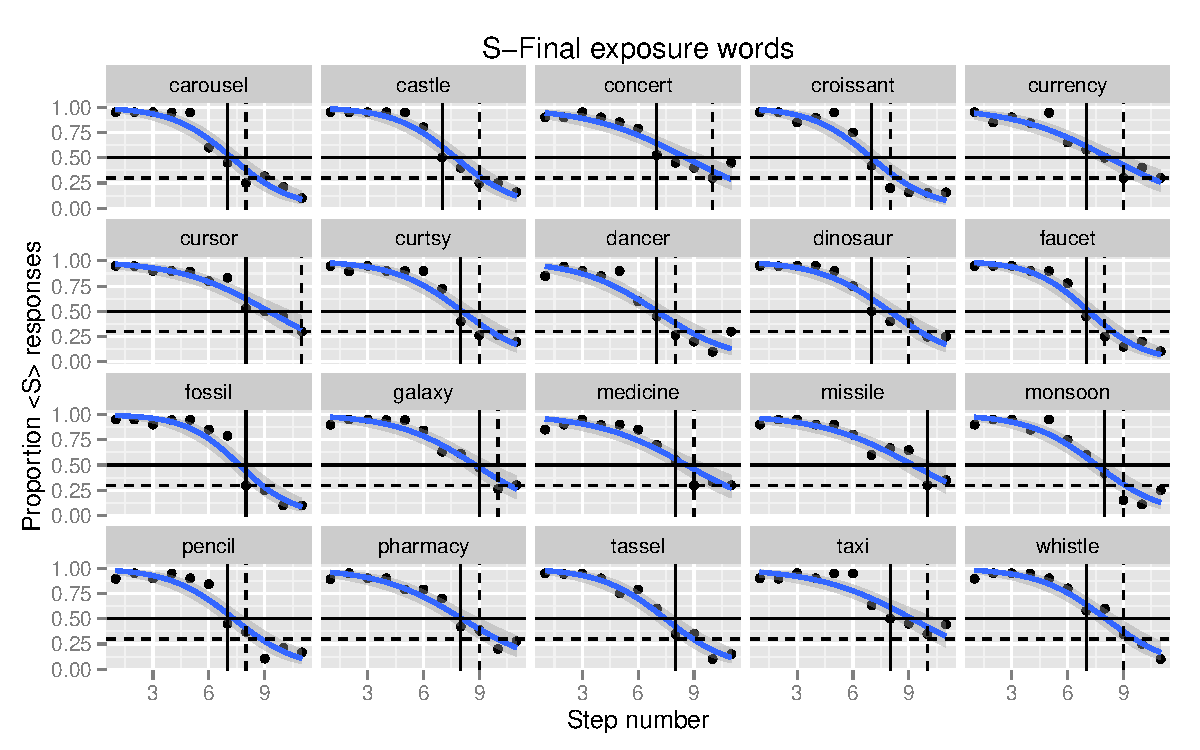
\includegraphics[width=\textwidth]{sfinalpretest.pdf}
\caption{Proportion of word-responses for /s/-final exposure words. Solid lines represent Experiment 1 selection criteria (50\% word-response rate) and dashed lines represent Experiment 2 selection criteria (30\% word-response rate).  Dots are averaged word-response across subjects, and the blue line is a binomial model constructed from the responses}
\end{figure}

\subsubsection{Procedure}

Participants in the experimental conditions completed two tasks, an exposure task and a categorization task.  
The exposure task was a lexical decision task, where participants heard auditory stimuli and were instructed to respond with either "word" if they thought what they heard was a word or "nonword" if they didn't think it was a word.  
The buttons corresponding to "word" and "nonword" were counterbalanced across participants. Trial order was pseudorandom, with no critical or control items appearing in the first six trials, and no critical or control trials in a row, but random otherwise, following \citet{Reinisch2013}.

In the categorization task, participants heard an auditory stimulus and had to categorize it as one of two words, differing only in the onset sibilant (s vs sh).  
The buttons corresponding to the words were counterbalanced across participants.  
The six most ambiguous steps of the minimal pair continua were used with seven repetitions each, giving a total of 168 trials.
Participants were instructed that there would two tasks in the experiment, and both tasks were explained at the beginning to remove experimenter interaction between exposure and categorization.  

Participants were assigned to one of four conditions. 
Two of the conditions exposed participants to only criticall items that began with /s/, and the other two exposed them to only critical items that had an /s/ in the onset of the final syllable, giving a consistent 200 trials in all exposure phases with control and filler items shared across all participants. 
Additionally participants in half the conditions received additional instructions that the speaker's "s" sounds were sometimes ambiguous, and to listen carefully to ensure correct responses in the lexical decision.

\subsection{Results}

\subsubsection{Control experiment}

Responses with reaction times less than 200 ms or greater than 2500 ms were excluded from analyses. 
A logistic mixed effects models was fit with Subject and Continua as random effects and Step as a fixed effect with by-Subject and by-Item random slopes for Step. 
The intercept was not significant ($\beta = 0.43, SE = 0.29, z = 1.5, p = 0.13$), and Step was significant ($\beta = -2.61, SE = 0.28, z = -9.1, p < 0.01$).

\subsubsection{Exposure}

Trials with nonword stimuli and responses faster than 200 ms or slower than 2500 ms were excluded from analysis. 
Performance on the exposure task was high overall, with accuracy on filler trials averaging 92\%.  
Word response rates for each of the four conditions did not differ significantly from each other, though S-Final/No Attention participants had a slightly higher average rate of 81\% (SD= 17\%) than the other conditions (S-Final/Attention: mean = 74\%, SD = 18\%; S-Initial/No Attention: mean = 74\%, SD = 27\%; S-Initial/Attention: mean = 76\%, SD = 23\%). 
A logistic mixed effects model with accuracy as the dependent variable was fit with fixed effects for trial type (Filler, S, SH), Attention (No Attention, Attention), Exposure Type (S-Initial, S-Final) and their interactions. 
The random effect structure was as maximally specified as possible with random effects for Subject and Word, and by-Subject random slopes for trial type and by-Word random slopes for Attention. 
The only fixed effects that were significant were a main effect of trial type for /s/ trials compared to filler trials ($\beta = -1.71, SE = 0.43, z = -3.97, p < 0.01$) and a main effect of Attention ($\beta = 0.76, SE = 0.38, z = 2.02,   p = 0.04$).  
Trials containing an ambiguous /s/ were less likely to be responded to as a word, and participants instructed to pay attention to /s/ were more likely to correctly respond to words in general.

\subsubsection{Categorization}

Responses with reaction times less than 200 ms or greater than 2500 ms were excluded from analyses. 
Participants were excluded if their initial estimated cross over point for the continuum lay outside of the 6 steps presented (2 participants).  
A logistic mixed effects model was constructed with Subject and Continua as random effects and continua Step as random slopes, with 0 coded as a /\textesh/ response and 1 as a /s/ response.  Fixed effects for the model were Step, Exposure Type, Attention and their interactions.

\begin{figure*}[!ht]
\caption{Proportion /s/ response along the 6 step continua as a function of Exposure Type and Attention in Experiment 1.    In the S-Final condition, participants in the Attention condition showed a larger perceptual learning effect than those in the No Attention condition.  In the S-Initial condition, there were no differences in perceptual learning between the Attention conditions. Error bars represent 95\% confidence intervals.}
\label{fig:exp1categ}
\begin{center}
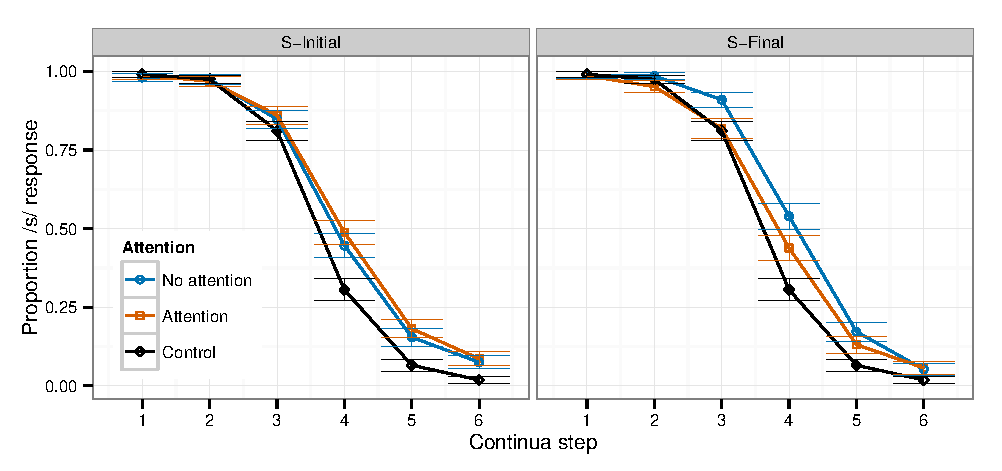
\includegraphics[width=\textwidth]{graphs/exp1_categresults}
\end{center}
\end{figure*}

There was a significant effect for the intercept ($\beta = 0.83, SE = 0.31, z = 2.6, p < 0.01$), indicating that participants categorized more of the continua as /s/ in general.  There was also a significant main effect of Step ($\beta = -2.10, SE = 0.20, z = -10.3, p < 0.01$), and a significant interaction between Exposure Type and Attention ($\beta = -0.93, SE = 0.43, z = -2.14, p = 0.03$).  There was a marginal main effect of Exposure Type ($\beta =0.58, SE = 0.30, z = 1.8, p = 0.06$).  

These results are shown in Figure~\ref{fig:exp1categ}.  
The solid lines show the control participants' categorization function across the 6 steps of the continua.  
The error bars show within-subject 95\% confidence intervals at each step.  
When exposed to ambiguous /s/ tokens in the first syllables of words, participants show a general expansion of the /s/ category, but no differences in behaviour if they are warned about ambiguous /s/ productions.  
However, when the exposure is to ambiguous /s/ tokens later in the words, we can see differences in behaviour beyond the general /s/ category expansion.  
Participants not warned of the speaker's ambiguous tokens categorized more of the continua as /s/ than those who were warned of the speaker's ambiguous /s/ productions.

\begin{figure*}[!ht]

\caption{Correlation of crossover point in categorization with the proportion of word responses to critical items containing an ambiguous /s/ token.}\label{fig:exp1xover}
\begin{center}
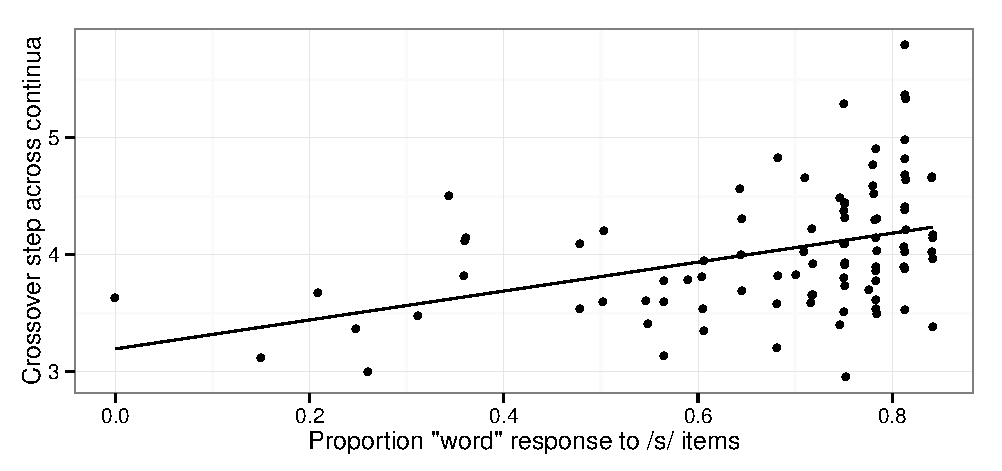
\includegraphics[width=\textwidth]{graphs/exp1_xoverwordresp}
\end{center}
\end{figure*}

As an individual predictor of participants' performance we took the proportion critical word endorsements and compared these values to the estimated cross-over points. 
The crossover point was determined from the Subject random effect in the logistic mixed effects model \citep{Kleber2011}. 
There was a significant positive correlation between a participant's tolerance for the ambiguous exposure items and their crossover point on the continua ($r = 0.39, t (90) = 4, p < 0.01$), shown in Figure~\ref{fig:exp1xover}.

An ANOVA with cross-over point as the independent variable and word endorsement rate, Exposure Type, Attention and their interactions, found only a main effect of word endorsement rate ($F(1,89) = 17.82, p < 0.01$), suggesting that listeners in different conditions were not affected differently from one another.

\subsection{Discussion}

Perceptual learning effects in this experiment were robust across continua and experimental conditions, indicating the general automaticity of perceptual adaptation, but the degree of adaptation differed across conditions. 
Differences in attention only had an effect in the S-Final conditions, which replicates earlier findings that the effect of attention increased as the position of the ambiguous sound moved toward the end of the word \cite{Pitt2012}.  
The initial sound of a word is already a prominent position and listeners focus on the initial sounds to narrow the set of possible words they might be hearing. Later in a word, expectations for particular words given the preceding phonetic content would be greater, so directed attention on the phonetic detail shows a clear effect.  
That attention affected perceptual learning at all suggests that the adaptation is not wholly automatic and there is some degree of listener control.

The threshold for stimuli selection differed from that in previous studies. The closest study to this one used 70\% of word responses in the pretest as the threshold for selection \citep{Reinisch2013}.  In that study, the lowest critical word endorsement rates in the exposure phase were 17 out of 20 (85\%).  In contrast, this experiment used 50\% as the threshold and had correspondingly lower word endorsement rates (mean = 76\%, sd = 22\%).  Interestingly, despite the lower word endorsement rates and the less canonical stimuli used, perceptual learning effects remained robust, which raises the question, can perceptual learning occur from stimuli that are farther from canonical productions than even the ones used in this experiment?

\section{Experiment 2}

Experiment 2 follows up on Experiment 1 by using stimuli that are farther from the canonical productions of the /s/ critical words.  If the correlation from Experiment 1 holds, we expect to see lower word endorsement rates and lower (or perhaps non-existent) perceptual learning effects.

\subsection{Methodology}

This experiment followed an identical methodology as experiment 1, except that the step along the /s/-/\textesh/ continua chosen as the ambiguous sound had a different threshold.  For this experiment, 30\% identification as the /s/ word was used the threshold. The average step chosen for /s/-initial words was 7.3 ($SD = 0.8$), and for /s/-final words the average step was 8.9 ($SD = 0.9$).

\subsection{Results}

\subsubsection{Exposure}

Trials with nonword stimuli and responses faster than 200 ms or slower than 2500 ms were excluded from analysis. 
Performance on the exposure task was high overall, with accuracy on filler trials averaging 92\%.  
An ANOVA of critical word endorsement rates revealed a marginal effect of Exposure Type ($F(1,92) = 3.86, p = 0.05$), with participants in the S-Final conditions having lower word endorsement rates (S-Final/Attention: mean = 56\%, sd = 30%; S-Final/No Attention: mean = 52\%, sd = 25\%) than participants in the S-Initial conditions (S-Initial/Attention: mean = 68\%, sd = 25\%; S-Initial/No Attention: mean = 61\%, sd = 23\%).
A logistic mixed effects model with accuracy as the dependent variable was fit with fixed effects for trial type (Filler, S, SH), Attention (No Attention, Attention), Exposure Type (S-Initial, S-Final) and their interactions. 
The random effect structure was as maximally specified as possible with random effects for Subject and Word, and by-Subject random slopes for trial type and by-Word random slopes for Attention. 
The only fixed effect that was significant were a main effect of trial type for /s/ trials compared to filler trials ($\beta = -2.51, SE = 0.46, z = -5.35, p < 0.01$).

\subsubsection{Categorization}

Responses with reaction times less than 200 ms or greater than 2500 ms were excluded from analyses. 
Participants were excluded if their initial estimated cross over point for the continuum lay outside of the 6 steps presented (2 participants).  
A logistic mixed effects model was constructed with Subject and Continua as random effects and continua Step as random slopes, with 0 coded as a /\textesh/ response and 1 as a /s/ response.  Fixed effects for the model were Step, Exposure Type, Attention and their interactions.

\begin{figure*}[!ht]
\caption{Proportion /s/ response along the 6 step continua as a function of Exposure Type and Attention in Experiment 1.    In the S-Final condition, participants in the Attention condition showed a larger perceptual learning effect than those in the No Attention condition.  In the S-Initial condition, there were no differences in perceptual learning between the Attention conditions. Error bars represent 95\% confidence intervals.}
\label{fig:exp2categ}
\begin{center}
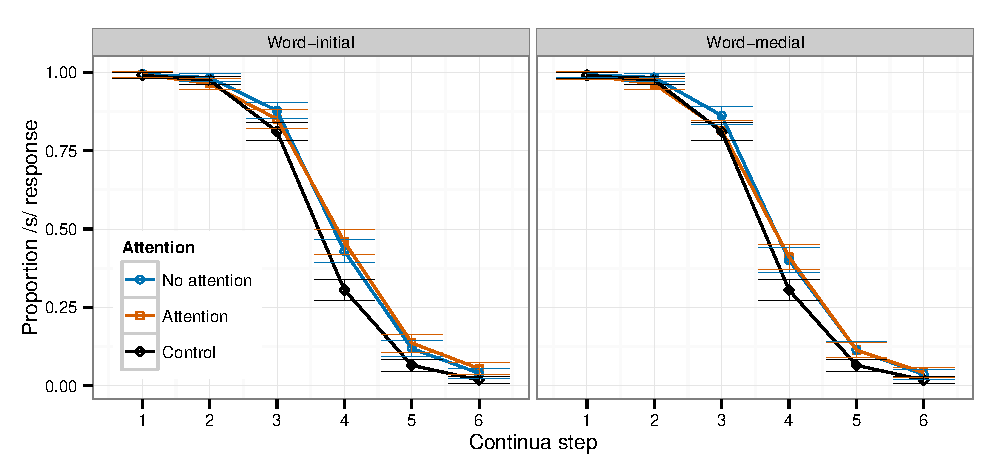
\includegraphics[width=\textwidth]{graphs/exp2_categresults}
\end{center}
\end{figure*}

There was a significant effect for the Intercept ($\beta = 1.01, SE = 0.38, z = 2.6, p < 0.01$), indicating that participants categorized more of the continua as /s/ in general.  There was also a significant main effect of Step ($\beta = -2.67, SE = 0.23, z = -11.2, p < 0.01$).  There were no other significant main effects or interactions, though an interaction between Step and Attention trended toward significant ($\beta = 0.35, SE = 0.21, z = 1.6, p = 0.09$).

\begin{figure*}[!ht]

\caption{Correlation of crossover point in categorization with the proportion of word responses to critical items containing an ambiguous /s/ token.}\label{fig:exp2xover}
\begin{center}
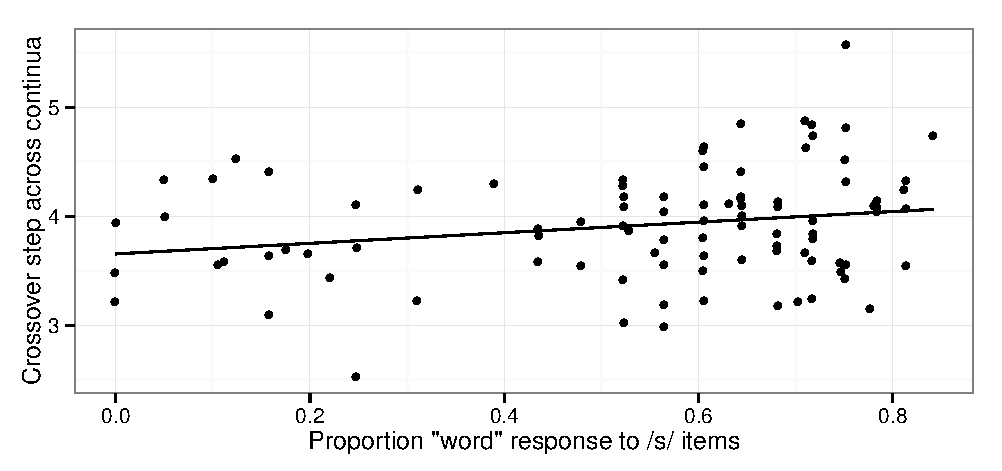
\includegraphics[width=\textwidth]{graphs/exp2_xoverwordresp}
\end{center}
\end{figure*}

As in Experiment 1,  the proportion critical word endorsements was calculated for each subject and assessed for correlation with participants' crossover points. There was a significant positive correlation between a participant's tolerance for the ambiguous exposure items and their crossover point on the continua ($r = 0.22, t (92) = 2.25, p = 0.02$), shown in Figure~\ref{fig:exp2xover}.  

\section{Groups results across experiments}

To see what degree the stimuli used had an effect on perceptual learning, the data from Experiment 1 and Experiment 2 were pooled and analyzed identically as above, but with Experiment and its interactions as fixed effects.  In the logistic mixed effects model, there was significant main effects for Intercept ($\beta = 1.00, SE = 0.36, z = 2.7, p < 0.01$) and Step ($\beta = -2.64, SE = 0.21, z = -12.1, p < 0.01$), and a significant two-way interaction between Experiment and Step ($\beta = 0.51, SE = 0.20, z = 2.5, p = 0.01$), and a marginal four-way interaction between Step, Exposure Type, Attention and Experiment ($\beta = 0.73, SE = 0.42, z = 1.7, p = 0.08$).  These results can be seen in Figure~\ref{fig:exp12categ}.  The four-way interaction can be seen in S-Final/No Attention conditions across the two experiments, where Experiment 1 has a significant difference between the Attention and No Attention condition, but Experiment 1 does not.  The two-way interaction between Experiment and Step and the lack of a main effect for Experiment potentially suggests that while the category boundary was not significantly different across experiments, the slope of the categorization function was.

\begin{figure*}[!ht]
\caption{Proportion /s/ response along the 6 step continua as a function of Exposure Type and Attention in Experiment 1. Error bars represent 95\% confidence intervals.}
\label{fig:exp12categ}
\begin{center}
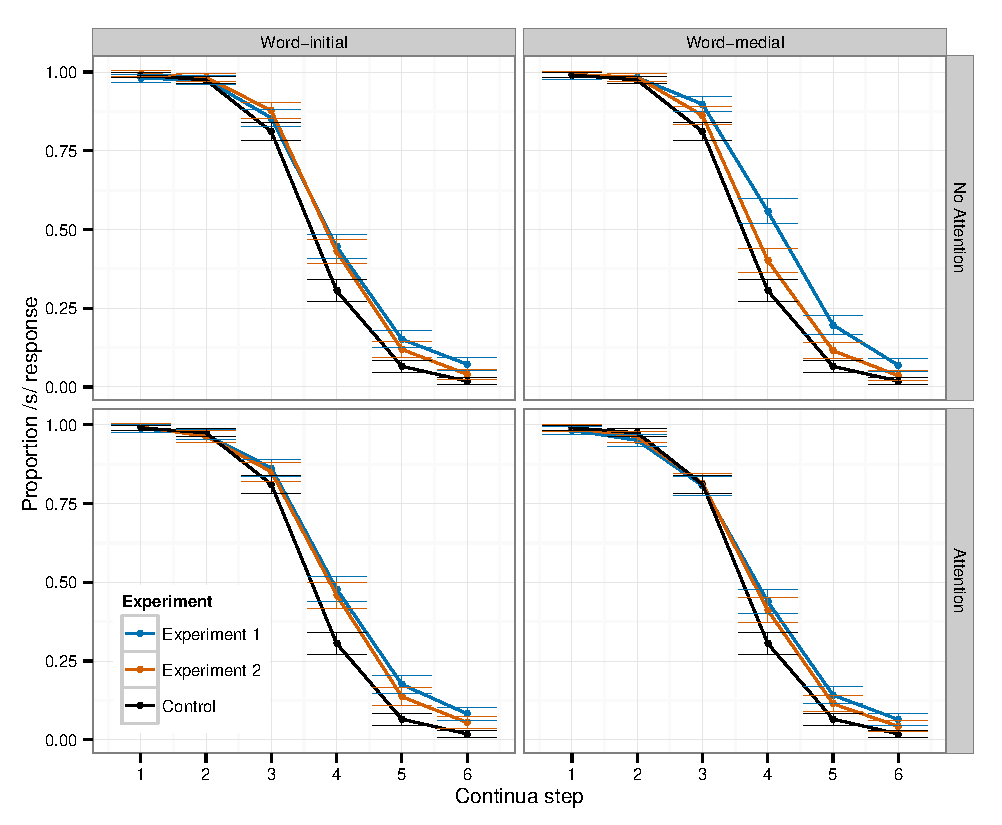
\includegraphics[width=\textwidth]{graphs/exp12_categresults}
\end{center}
\end{figure*}

To see if there was a difference with the Experiment 1 in how word endorsement rates affected crossover points, the data was pooled for the two experiments.  An ANOVA with cross-over point as the independent variable and word endorsement rate, Exposure Type, Attention, Experiment and their interactions, found a main effect of word endorsement rate ($F(1,185) = 21.82, p < 0.01$) and marginal interaction between word endorsement rates and Experiment ($F(1, 185) = 3.11, p = 0.07$).

\section{General discussion}

Perceptual learning was found across all experimental conditions. Attention only had effect on perceptual learning in the S-Final condition of Experiment 1.  
%The differences in between experiments appears to not be in the location of the new boundary, but rather in the slope of the categorization funcion.  In Experiment 1, where the ambiguous tokens are halfway between /s/ and /\textesh/, the slope 

Compared to Experiment 1, Experiment 2 had a weaker, yet still significant, correlation between critical word endorsement rates and crossover boundary points, suggesting that although the stimuli used in Experiment 2 were farther from the canonical production, they did not shift the category boundary as much as the stimuli in Experiment 1.  While neither attention or position of the ambiguous sound in the word had an effect on the correlation, the distance from the canonical production did.  This potentially suggests that the degree to which a category is shifted is inversely related to its distance.  Or perhaps more likely, the distance is inversely related to its goodness or plausibility that the ambiguous sound was indeed meant to be an /s/.

The correlation between word response rate in the exposure phase and the category boundary in categorization phase across both experiments raises two possible explanations. 
In a causal interpretation between exposure and categorization, as each ambiguous sound is linked to a word and a phonetic category, the distribution for that category (for that particular speaker) is updated.
 Participants who linked more of the ambiguous sound to the /s/ category updated their perceptual category for /s/ more. 
This explanation fits within a larger neo-generative model of spoken language processing \citep{Pierrehumbert2002}.  
A non-causal story is also plausible:  the correlation may reveal individual differences on the part of the participants, where some participants are more adaptable or tolerant of variability than others, leading to greater degrees of perceptual adaptation. 
The lack of learning with nonwords \citep{Norris2003} makes the latter interpretation particularly appealing.